% === C06 - Conmutación basica de tareas ===
% David Alejandro Gonzalez Marquez
% dmarquez@dc.uba.ar / fokerman@gmail.com
% https://github.com/fokerman/Orga2Course

\documentclass[aspectratio=169]{beamer}
% \documentclass[handout]{beamer}

% % % Packages
\usepackage[sfdefault]{AlegreyaSans}
\usepackage{inconsolata}
\usepackage{multicol}
\usepackage{multirow}
\usepackage[spanish]{babel}
\usepackage[utf8]{inputenc}
\usepackage{enumerate}
\usepackage{color}
\usepackage{xcolor}
\usepackage[absolute,overlay]{textpos}
  \setlength{\TPHorizModule}{1mm}
  \setlength{\TPVertModule}{1mm}
\usepackage{framed}
\usepackage{mfirstuc} % para poner en mayusculas la primer letra
\usepackage{xspace} % para crear espacios en comandos 
\usepackage{pbox}
\usepackage{tikz}
\usepackage{mathabx}

% % % Beamer config
\usetheme{Pittsburgh}
\usecolortheme[rgb={1,0.48,0.0}]{structure}
\setbeamercolor{block title}{fg=white,bg=verdeuca}
\xdefinecolor{verdeuca}{rgb}{0.0,0.48,0.54}
\xdefinecolor{naranjauca}{rgb}{1,0.48,0.0}
\setbeamercolor{palette quaternary}{fg=white,bg=verdeuca}
\setbeamertemplate{title page}[default][colsep=-4bp, rounded=true] % remove title shadow
\setbeamertemplate{frametitle}[default][colsep=-2bp, shadow=false] % remove frame title shadow
\setbeamertemplate{navigation symbols}{} % remove navigation symbols
\beamertemplatenavigationsymbolsempty

% % % Colors
\definecolor{AzulClaro}{rgb}{.31,.506,.741}
\definecolor{Gris}{gray}{0.8}
\definecolor{Celeste}{rgb}{.255,.41,.884}
\definecolor{Rojo}{rgb}{1, 0, 0}
\definecolor{a}{rgb}{0.0, 0.53, 0.74}
\definecolor{r}{rgb}{0.89, 0.0, 0.13}
\definecolor{v}{rgb}{0.0, 0.5, 0.0}
\definecolor{y}{rgb}{0.0, 0.5, 0.5}
\definecolor{rojo}{HTML}{F1521B}
\definecolor{verde}{HTML}{80CD29}
\definecolor{amarillo}{HTML}{FABC09}
\definecolor{azul}{HTML}{00ADF1}

% % % Rename
\newcommand{\tab}[0]{\hspace{15pt}}

% % % Blocks
\setbeamercolor{block body}{fg=black, bg=black!10}
\setbeamercolor{block title}{fg=black, bg=black!20}
\setbeamercolor{coloredboxstuffNaranja}{fg=naranjauca,bg=black!10} %% PARA LOS BOX
\setbeamercolor{coloredboxstuffVerde}{fg=verdeuca,bg=black!10} %% PARA LOS BOX

% % % Start

\title{\Huge Conmutación básica de tareas}
\subtitle{Programación de Sistemas Operativos}
      
\author{David Alejandro González Márquez}
\institute{Departamento de Computación\\
Facultad de Ciencias Exactas y Naturales\\
Universidad de Buenos Aires}
\date{}

\begin{document}

\frame[plain]{\titlepage}

\begin{frame}
    \frametitle{Introducci\'on}
    \Large \textcolor{naranjauca}{Tareas}
    \normalsize
    \vspace{0.5cm}
    \begin{itemize}
    \large 
    \setlength\itemsep{0.5cm}
    \item[-]<2-> Una \emph{tarea} es una unidad de trabajo que el procesador\\  puede \textbf{ejecutar}, \textbf{desalojar} e \textbf{intercambiar} por otra.
    \item[-]<3-> La tarea ejecuta una instancia de un programa y se puede ver\\  como un \textbf{contexto de ejecución}.
    \item[-]<4-> La arquitectura provee un mecanismo nativo para: 
    \begin{itemize}
    \large 
    \item[-] salvar el contexto de una tarea,
    \item[-] comenzarla a ejecutar o
    \item[-] conmutarla con otra.
    \end{itemize}
    \end{itemize}
\end{frame}

\begin{frame}
    \frametitle{Introducci\'on}
    \large Una tarea est\'a compuesta por:
    \vspace{0.4cm}
    \pause
    \begin{enumerate}
        \item Espacio de ejecuci\'on:\only<4->{\textcolor{naranjauca}{$\rightarrow$\textbf{Memoria}}}
        \begin{itemize}
        \large
        \vspace{0.1cm}
        \item[-] Segmento de c\'odigo.
        \vspace{0.1cm}
        \item[-] Segmento de datos/pila (uno o varios).
        \vspace{0.1cm}
        \item[-] Mapa de páginas (\texttt{CR3}, con paginación esta activa).
        \end{itemize}
        \vspace{0.4cm}
        \pause
        \item Segmento de estado (TSS):\only<5->{\textcolor{naranjauca}{$\rightarrow$\textbf{Contexto}}}
        \begin{itemize}
        \vspace{0.1cm}
        \large
        \item[-] Almacena el estado de la tarea (su contexto) para poder reanudarla.
        \begin{itemize}
        \large
        \vspace{0.05cm}
        \item[-] Registros de propósito general y selectores de segmento.
        \item[-] Flags, \emph{CR3}, \emph{LDTR} y Pilas de niveles de privilegio superior.
        \end{itemize}
        \end{itemize}
    \end{enumerate}
\end{frame}

\begin{frame}
\frametitle{Introducci\'on: Estructura}
    \begin{center}Estructura de una tarea\end{center}
    \vspace{-0.5cm}
    \begin{figure}[ht!]
    \centering
    \includegraphics[scale=0.9]{img/Structure_Task.pdf}
    \end{figure}
\end{frame}

\begin{frame}
\frametitle{TSS: Task-State Segment}
    \begin{textblock}{100}(4,10) \only<1->{ \includegraphics[scale=0.52]{img/TSS.pdf} } \end{textblock}  % Memoria y CPU
    \begin{textblock}{75}(72,14)
        \begin{itemize}
        \item<2->[-] Una tarea est\'a identificada por un selector de segmento de \texttt{TSS}.
        \vspace{0.5cm}
        \item<3->[-] La TSS debe estar descripta en la GDT del mismo modo que se describen los segmentos de c\'odigo y datos.
        \vspace{0.5cm}
        \item<4->[-] El registro Task Register (TR) contiene selector de segmento de TSS de la tarea que se est\'a ejecutando actualmente.
        \end{itemize}
    \end{textblock}
\end{frame}
    
\begin{frame}
\frametitle{TSS: Descriptor de TSS}
\vspace{-0.4cm}
\begin{figure}[ht!]
	\centering
	\includegraphics[scale=0.8]{img/TSS_descriptor.pdf}
\end{figure}
\end{frame}

\begin{frame}
\frametitle{TSS: Relación entre Task Register y GDT y TSS de la tarea acutal}
\vspace{-0.1cm}
\begin{figure}[ht!]
	\centering
	\includegraphics[scale=0.7]{img/Task_Register_ref.pdf}
\end{figure}
\end{frame}

\begin{frame}
    \frametitle{Intercambio de tareas}
    \begin{textblock}{100}(4,14) \only<1->{\includegraphics[scale=1]{img/conmutacion-layer1.pdf}} \end{textblock}  % Memoria y CPU
    \begin{textblock}{100}(4,14) \only<2->{\includegraphics[scale=1]{img/conmutacion-layer2.pdf}} \end{textblock}  % GDT
    \begin{textblock}{100}(4,14) \only<3->{\includegraphics[scale=1]{img/conmutacion-layer3.pdf}} \end{textblock}  % TSS
    \begin{textblock}{100}(4,14) \only<4->{\includegraphics[scale=1]{img/conmutacion-layer10.pdf}} \end{textblock} % CODIGO
    
    \begin{textblock}{100}(4,14) \only<5->{\includegraphics[scale=1]{img/conmutacion-layer11.pdf}} \end{textblock} % SELECTOR
    \begin{textblock}{100}(4,14) \only<6-7>{\includegraphics[scale=1]{img/conmutacion-layer5.pdf}} \end{textblock}  % GDT TSS2
    \begin{textblock}{100}(4,14) \only<7->{\includegraphics[scale=1]{img/conmutacion-layer9.pdf}} \end{textblock}  % CONTENIDO TSS2
    
    \begin{textblock}{100}(4,14) \only<8-11|handout:0>{\includegraphics[scale=1]{img/conmutacion-layer13.pdf}} \end{textblock} % DISABLE
    \begin{textblock}{100}(4,14) \only<8-10|handout:0>{\includegraphics[scale=1]{img/conmutacion-layer14.pdf}} \end{textblock} % TR TSS1
    \begin{textblock}{100}(4,14) \only<8-10|handout:0>{\includegraphics[scale=1]{img/conmutacion-layer12.pdf}} \end{textblock} % FLECHA TR
    \begin{textblock}{100}(4,14) \only<9-11>{\includegraphics[scale=1]{img/conmutacion-layer4.pdf}} \end{textblock}  % GDT TSS1
    
    \begin{textblock}{100}(4,14) \only<11-11>{\includegraphics[scale=1]{img/conmutacion-layer6.pdf}} \end{textblock}  % FLECHA TSS1
    \begin{textblock}{100}(4,14) \only<11->{\includegraphics[scale=1]{img/conmutacion-layer8.pdf}} \end{textblock}  % CONTENIDO TSS1
    \begin{textblock}{100}(4,14) \only<11-12|handout:0>{\includegraphics[scale=1]{img/conmutacion-layer13.pdf}} \end{textblock} % DISABLE
    \begin{textblock}{100}(4,14) \only<11-11|handout:0>{\includegraphics[scale=1]{img/conmutacion-layer17.pdf}} \end{textblock} % CONTEXTO
    
    \begin{textblock}{100}(4,14) \only<12-14|handout:0>{\includegraphics[scale=1]{img/conmutacion-layer5.pdf}} \end{textblock}  % GDT TSS2
    \begin{textblock}{100}(4,14) \only<13-14|handout:0>{\includegraphics[scale=1]{img/conmutacion-layer13.pdf}} \end{textblock} % DISABLE
    \begin{textblock}{100}(4,14) \only<13-14>{\includegraphics[scale=1]{img/conmutacion-layer7.pdf}} \end{textblock}  % FLECHA TSS2
    \begin{textblock}{100}(4,14) \only<13-14|handout:0>{\includegraphics[scale=1]{img/conmutacion-layer15.pdf}} \end{textblock} % TR TSS2
    \begin{textblock}{100}(4,14) \only<14-14|handout:0>{\includegraphics[scale=1]{img/conmutacion-layer17.pdf}} \end{textblock} % CONTEXTO
    
    \begin{textblock}{100}(4,14) \only<15-|handout:0>{\includegraphics[scale=1]{img/conmutacion-layer13.pdf}} \end{textblock} % DISABLE
    \begin{textblock}{100}(4,14) \only<15-|handout:0>{\includegraphics[scale=1]{img/conmutacion-layer18.pdf}} \end{textblock} % RUN
    
%     \begin{textblock}{100}(4,12) \only<13-14->{\includegraphics[scale=1]{img/conmutacion-layer16.pdf}} \end{textblock} % TR
    \begin{textblock}{200}(98,25)
    \small 
    \begin{enumerate}
    \item<5->  Determinar y validar TSS a ejecutar
    \item<8->  Identificar la tarea en ejecución
    \item<10->  Guardar el contexto actual a memoria
    \item<12-> Cargar el nuevo contexto de memoria
    \item<15-> Continuar la ejecución desde \texttt{CS:EIP}
    \end{enumerate}
    \end{textblock}
\end{frame}

\begin{frame}
\frametitle{Conmutaci\'on de Tareas: Tarea Inicial}
\begin{enumerate}
	\item<2-> Siempre que se salta a una tarea, hay un cambio de contexto, \textbf{¡Siempre!}
	\vspace{0.4cm}
	\item<3-> El procesador guarda el contexto actual de la tarea (identificada en TR)\\ y carga el contexto de la tarea a la cual se est\'a saltando.
	\vspace{0.4cm}
	\item<4-> Entonces,\\ ?`qu\'e pasa la primera vez?\\ ?`Qu\'e pasa cuando se salta a la primera tarea?\\ ?`Qu\'e valor contiene TR?\\ ?`D\'onde se guarda el contexto?
	\vspace{0.4cm}
	\item<5-> Hay que crear una \textbf{tarea inicial} para proveer una TSS en donde el procesador pueda guardar el contexto actual. \textcolor{verdeuca}{Esta tarea inicial tiene este \'unico prop\'osito.}
	\vspace{0.4cm}
\end{enumerate}
\end{frame}

\begin{frame}
\frametitle{Conmutaci\'on de Tareas: Checklist}
\begin{enumerate}
	\item Al iniciar las tareas:
		\begin{itemize}
		\item<1-> completar \textbf{EIP}
		\item<2-> completar \textbf{ESP} y  \textbf{EBP}
		\item<3-> completar selectores de segmento \textbf{CS}, \textbf{DS}, $\cdots$ ,\textbf{SS} \only<9->{{\scriptsize \textcolor{verdeuca}{(recordar RPL)}}}
		\item<4-> completar \textbf{CR3}
		\item<5-> completar \textbf{EFLAGS} \only<9->{\textcolor{verdeuca}{(*)}}
		\end{itemize}
	\vspace{0.4cm}
	\item<6-> Al saltar por primera vez a una tarea:
		\begin{itemize}
		\item<6-> tener un descriptor en la GDT de la tarea inicial
		\item<7-> tener un descriptor en la GDT de la tarea a saltar
		\item<8-> tener en \textbf{TR} alg\'un valor v\'alido (tarea inicial)
		\end{itemize}
\end{enumerate}
\end{frame}

\begin{frame}
\frametitle{Conmutaci\'on de Tareas: EFLAGS}
    \vspace{-0.5cm}
    \begin{figure}[ht!]
    \centering
    \includegraphics[scale=0.8]{img/EFLAGS.pdf}
    \end{figure}
    \footnotesize
    \begin{columns}[c]
    \column{0.39\textwidth}
    \begin{itemize}
    \item[] \large \textbf{EFLAGS por defecto}\\ \textcolor{naranjauca}{\texttt{0x00000002}}
    \end{itemize}
    \column{0.65\textwidth}
    \begin{itemize}
    \item[] \large \textbf{EFLAGS con Interrupciones habilitadas}\\ \textcolor{naranjauca}{\texttt{0x00000202}}
    \end{itemize}
    \end{columns}
\end{frame}

\begin{frame}[fragile]
    \frametitle{Conmutaci\'on de Tareas: Instrucciones}
    \begin{itemize}
        \item[-] Cargar la tarea inicial en el \verb|TR|
    \end{itemize}
    \begin{verbatim}
            mov ax, <sel.init>
            ltr ax
    \end{verbatim}
    \pause
    \begin{itemize}
        \item[-] Saltar a la nueva tarea (intercambio)
    \end{itemize}
    \begin{verbatim}
            jmp <sel.task>:0
    \end{verbatim}
    \pause
    \vspace{0.5cm}
    \begin{tabular}{l|l|l}
    \texttt{<sel.init>} & \small \textbf{Tarea inicial}  & \small Primera tarea que se carga, destino del contexto de ejecución actual.\\
    \texttt{<sel.task>} & \small \textbf{Tarea a saltar} & \small Contexto de ejecución válido que se cargará en el procesador.\\
    \end{tabular}
\end{frame}

\begin{frame}[plain]
\Huge \textcolor{naranjauca}{Trabajo Práctico}
\end{frame}

\begin{frame}[t]
\frametitle{Trabajo Práctico}

En el TP se debe crear una tarea inicial y luego saltar a la tarea \emph{Idle}. Este ejercicio tiene el propósito de realizar un intercambio de tareas.
\pause
\small
\begin{block}{\small Pasos para saltar a la tarea \emph{Idle}}
\vspace{-0.3cm}
\begin{enumerate}
\setlength\itemsep{0pt}
\item<2-> Completar las entradas en la \texttt{GDT} para la \emph{tarea inicial} y la tarea Idle.
\item<3-> Completar la \texttt{TSS} de la tarea Idle:\\
\vspace{0.1cm}
\uncover<4->{\hspace{1cm} \textcolor{verdeuca}{\texttt{EIP} = \texttt{0x1A000}. Comienzo del código de la tarea Idle.}}\\
\uncover<5->{\hspace{1cm} \textcolor{verdeuca}{\texttt{CR3} = \texttt{0x27000}. El mismo mapa de paginación del \texttt{kernel}.}}\\
\uncover<6->{\hspace{1cm} \textcolor{verdeuca}{\texttt{ESP} = \texttt{0x27000}. Misma pila del Kernel.}}\\
\uncover<7->{\hspace{1cm} \textcolor{verdeuca}{\texttt{CS} = Selector de segmento de código de nivel cero.}}\\
\uncover<8->{\hspace{1cm} \textcolor{verdeuca}{\texttt{DS}$\cdots$\texttt{SS} = Selector de segmento de datos de nivel cero.}}\\
\uncover<9->{\hspace{1cm} \textcolor{verdeuca}{\texttt{EEFLAGS} = \texttt{0x202}. Interrupciones activas.}}\\
\item<10-> \small Escribir el código necesario para ejecutar la tarea \texttt{Idle}, es decir, saltar intercambiando las \texttt{TSS}, entre la \emph{tarea inicial} y la tarea \texttt{Idle}.\\
\vspace{0.1cm}
\uncover<11->{\hspace{1cm} \textcolor{verdeuca}{\texttt{mov ax, <selector de segmento de la tarea inicial>}}}\\
\uncover<12->{\hspace{1cm} \textcolor{verdeuca}{\texttt{ltr ax}}}\\
\uncover<13->{\hspace{1cm} \textcolor{verdeuca}{\texttt{jmp <selector de segmengo de la tarea Idle>:0}}}
\end{enumerate}
\vspace{-0.3cm}
\end{block}
\end{frame}

\begin{frame}[fragile]
    \frametitle{Bibliografía: Fuentes y material adicional}
    \begin{itemize}
    \item Convenciones de llamados a función en x86: \\
    \url{https://en.wikipedia.org/wiki/X86_calling_conventions}
    \item Notas sobre System V ABI: \\
    \url{https://wiki.osdev.org/System_V_ABI}
    \item Documentación de NASM: \\
    \url{https://nasm.us/doc/}
    \item Artículo sobre el flag \texttt{-pie}: \\
    \url{https://eklitzke.org/position-independent-executables}
    \item Documentación de System V ABI: \\
    \url{https://uclibc.org/docs/psABI-x86_64.pdf}
    \item Manuales de Intel: \\
    \url{https://software.intel.com/en-us/articles/intel-sdm}
    \end{itemize}
\end{frame}

\begin{frame}[plain]
    \begin{center}
    \vspace{2cm}
    \huge ¡Gracias!\\
    \vspace{2cm}
    \normalsize Recuerden leer los comentarios al final de \\ este video por aclaraciones o fe de erratas.
    \end{center}
\end{frame}

\end{document}

% % % % % % % % % % % % % % % % % % % % % % %
% NOTAS SOBRE EL JUEGO DEL TRABAJO PRACTICO %
% Primer Cuatrimestre 2020                  %
% % % % % % % % % % % % % % % % % % % % % % %

\begin{frame}[plain]
\Huge \textcolor{naranjauca}{Game}
\end{frame}

\begin{frame}[fragile]
\frametitle{Game}
\begin{figure}[ht!]
	\centering
	\includegraphics[scale=0.57]{../../tps/tp3/enunciado/img/game.pdf}
\end{figure}
\pause
\begin{itemize}
\footnotesize
 \item Posición de los Jugadores: \texttt{Pos[player]}
 \item Pelotas restantes por jugador: \texttt{Life[player]}
 \item Puntos por jugador: \texttt{Count[player]}
 \item Posición de las pelotas por jugador: \texttt{TaskPos[player][task][xy]}
 \item Interpretación de las coordenadas: \texttt{TaskRef[player][task][xy]}
\end{itemize}
\end{frame}

\begin{frame}[fragile]
\frametitle{Game}
\begin{center}
\footnotesize
\begin{tabular}{c|c|c}
Jugador & Tecla & Acción \\
\hline
 \multirow{3}{*}{Jugador A} & \verb|w| & mover hacia arriba \\
                            & \verb|s| & mover hacia abajo \\
                            & \verb|z|, \verb|x|, \verb|c| & nueva pelota tipo 1, 2, 3\\
 \hline
 \multirow{3}{*}{Jugador B} & \verb|i| & mover hacia arriba \\
                            & \verb|k| & mover hacia abajo \\
                            & \verb|b|, \verb|n|, \verb|m| & nueva pelota tipo 1, 2, 3\\
 \hline
\end{tabular}
\end{center}
\pause
\textbf{Nueva tarea}:
\begin{enumerate}
 \item Buscar espacio libre donde crear la tarea
 \item Crear un nuevo mapa de memoria
 \begin{itemize}
  \item Identity Mapping primeros 4MB
  \item Copiar y mapear código
 \end{itemize}
 \item Completar información de estado
 \begin{itemize}
  \item Completar la posición dentro del mapa
  \item Agregar a la lista de tareas
 \end{itemize}
\end{enumerate}
\end{frame}

\begin{frame}[fragile]
\frametitle{Game \textbf{Syscalls} }
\begin{tabular}[h]{p{2.4cm}p{7.6cm}}
\normalsize \verb|talk| & \small \verb|in EAX|$=$\verb|0x80000001|\\
                        & \small \verb|in EBX|$=$\verb|char* m|\\
                        & \scriptsize Envia el mensaje en \verb|m|. (\verb|strlen(m)|$<$20) \\
\end{tabular}
\vspace{0.2cm}

\begin{tabular}[h]{p{2.4cm}p{7.6cm}}
\normalsize \verb|where| & \small \verb|in EAX|$=$\verb|0x80000002|\\
                         & \small \verb|out EBX|$=$\verb|uint32_t x|\\
                         & \small \verb|out ECX|$=$\verb|uint32_t y|\\
                         & \scriptsize  Retorna las coordenadas \verb|x| e \verb|y| de la pelota.
\end{tabular}
\vspace{0.2cm}

\begin{tabular}[h]{p{2.4cm}p{7.6cm}}
\normalsize \verb|setHandler| & \small \verb|in EAX|$=$\verb|0x80000003|\\
                              & \small \verb|in EBX|$=$\verb|f_handler_t* f|\\
                              & \scriptsize Registra la dirección de la función \emph{handler}.
\end{tabular}
\vspace{0.2cm}

\begin{tabular}[h]{p{2.4cm}p{7.6cm}}
\normalsize \verb|informAction| & \small \verb|in EAX|$=$\verb|0x8000FFFF|\\
                                & \small \verb|in EBX|$=$\verb|e_action action|\\
                                & \scriptsize Retornar al sistema desde la función \verb|handler|. \\
\end{tabular}
\end{frame}

\begin{frame}[plain]
\Huge \textcolor{naranjauca}{Scheduler}
\end{frame}

\begin{frame}[fragile]
\frametitle{Scheduler}
\begin{figure}[ht!]
    \begin{textblock}{100}(1,20)
    \begin{center}
    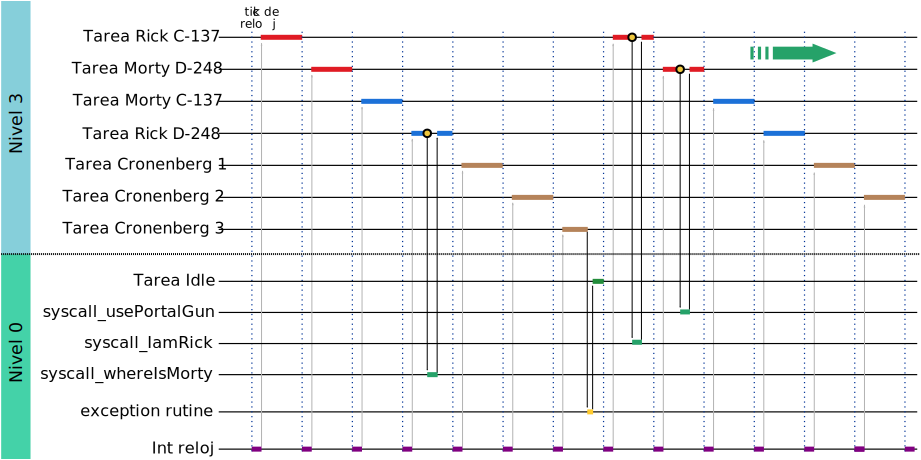
\includegraphics[scale=0.56]{../../tps/tp3/enunciado/img/sched_example.pdf}
    \end{center}
    \end{textblock}
\end{figure}
\end{frame}

\begin{frame}[fragile]
\frametitle{Scheduler}
\begin{figure}[ht!]
	\centering
	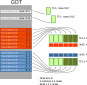
\includegraphics[scale=0.80]{img/figura_gdt_tp3.pdf}
\end{figure}
\end{frame}

\begin{frame}[fragile]
\frametitle{Scheduler}
    \begin{textblock}{100}(25,3)
    \begin{center}
    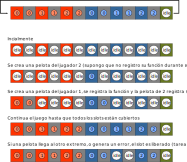
\includegraphics[scale=0.50]{img/figura_scheduler.pdf}
    \end{center}
    \end{textblock}
\end{frame}

\begin{frame}[fragile]
\frametitle{Modo Debug}
\begin{figure}[ht!]
	\centering
	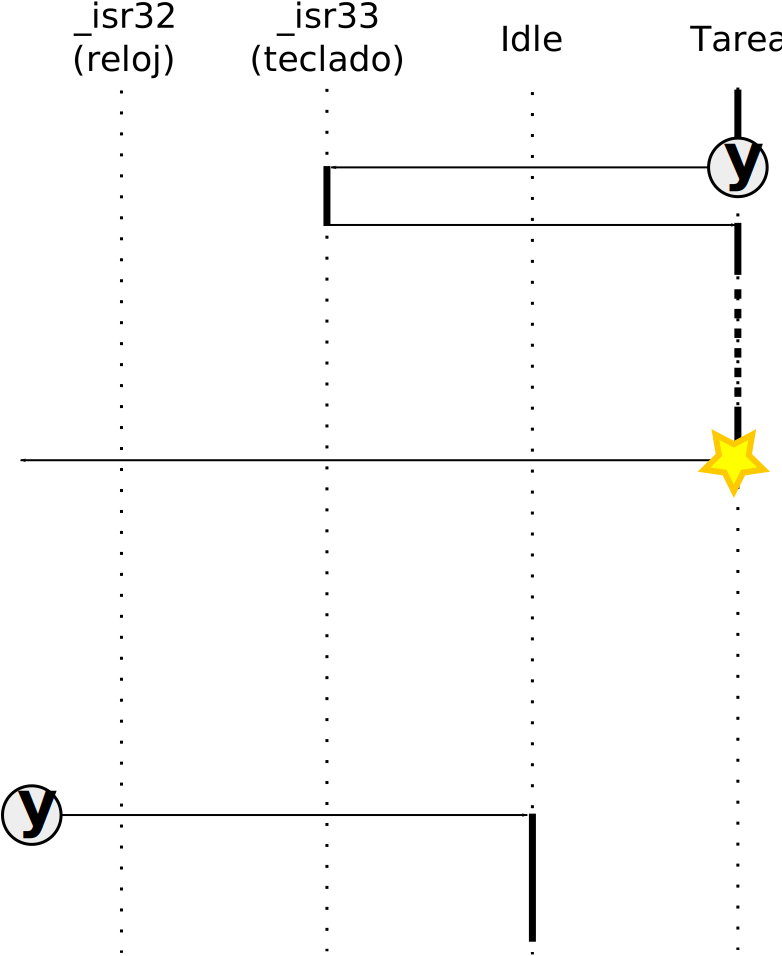
\includegraphics[scale=0.29]{img/figura_debug.pdf}
\end{figure}
\end{frame}

\begin{frame}[t]
\frametitle{El TP3}
\small
\vspace{-0.3cm}
\begin{block}{\small Ejercicio 7}
\vspace{-0.5cm}
\begin{enumerate}[a)]
\setlength\itemsep{0em}
\item Construir una función para inicializar las estructuras de datos del \emph{scheduler}.
\item Crear la función \texttt{sched\_nextTask()} que devuelve el índice en la \texttt{GDT} de la próxima tarea a ser ejecutada.
\item Modificar la rutina de interrupciones \texttt{0x47} para que implemente los distintos servicios del sistema.
\item Modificar el código necesario para que se realice el intercambio de tareas por cada ciclo de reloj.
El intercambio se realizará según indique la función \texttt{sched\_nextTask()}.
\item Modificar las rutinas de excepciones del procesador para que desalojen a la tarea que estaba corriendo y ejecuten la próxima.
\item Implementar el mecanismo de debugging indicando en pantalla la razón del desalojo de la tarea.
\end{enumerate}
\end{block}
\end{frame}

\begin{frame}[fragile]
\frametitle{Ayudas}
\normalsize
\begin{itemize}
    \item Leer una tecla
\end{itemize}
\scriptsize
\begin{verbatim}
xor eax, eax
in al, 60h
test al, 10000000b
jnz .fin
\end{verbatim}
\normalsize
\begin{itemize}
    \item Saltar a una tarea
\end{itemize}
\scriptsize
\begin{verbatim}
offset: dd 0
selector: dw 0
...
mov [selector], ax
jmp far [offset]
...
\end{verbatim}
\end{frame}

\begin{frame}[fragile]
\frametitle{Ayudas}
Rutina de atención de interrupciones para el reloj
\scriptsize
\begin{verbatim}
global _isr32
_isr32:
   pushad

   call pic_finish1

   call sched_nextTask

   str cx
   cmp ax, cx
   je .fin

      mov [selector], ax
      jmp far [offset]

   .fin:

   popad
 iret
\end{verbatim}
\end{frame}

\begin{frame}[fragile]
\frametitle{Ayudas}
\centering
\small
ASM para usar desde C (i386.h)
\scriptsize
\begin{verbatim}
void lcr0(unsigned int val)
unsigned int rcr0(void)
 
void lcr1(unsigned int val)
unsigned int rcr1(void)
 
void lcr2(unsigned int val)
unsigned int rcr2(void)
 
void lcr3(unsigned int val)
unsigned int rcr3(void)
 
void lcr4(unsigned int val)
unsigned int rcr4(void)
 
void tlbflush(void)
 
void ltr(unsigned short sel)
unsigned short rtr(void)
 
void breakpoint(void)
\end{verbatim}
\end{frame}

\begin{frame}[plain]
  \begin{center}
    \Huge{¿Preguntas?}
  \end{center}
\end{frame}

\end{document}
